\documentclass[11pt]{article}
\usepackage[scaled=0.92]{helvet}
\usepackage{geometry}
\geometry{letterpaper,tmargin=1in,bmargin=1in,lmargin=1in,rmargin=1in}
\usepackage[parfill]{parskip} % Activate to begin paragraphs with an empty line rather than an indent %\usepackage{graphicx}
\usepackage{amsmath,amssymb, mathrsfs, dsfont}
\usepackage{tabularx}
\usepackage[font=footnotesize,labelfont=bf]{caption}
\usepackage{graphicx}
\usepackage{xcolor}
%\usepackage[linkbordercolor ={1 1 1} ]{hyperref}
%\usepackage[sf]{titlesec}
\usepackage{natbib}
\usepackage{../../Tianpei_Report}
%\usepackage{appendix}
%\usepackage{algorithm}
%\usepackage{algorithmic}

%\renewcommand{\algorithmicrequire}{\textbf{Input:}}
%\renewcommand{\algorithmicensure}{\textbf{Output:}}



\begin{document}
\title{Lecture 1: Context-Free Grammar and related concepts}
\author{ Tianpei Xie}
\date{ Jun. 26th., 2022 }
\maketitle
\tableofcontents
\newpage
\allowdisplaybreaks
\section{Concepts and Terminology}
The basics of linguistic study is the grammar and terminologies. We summarize a list of basic grammar terms. \textbf{Context-free grammars} (a.k.a. \textbf{Phrase-Structure Grammars}) are the backbone of many formal models of the syntax of natural language (and, for that matter, of computer languages). As such, they play a role in many computational applications, including grammar checking, semantic interpretation, dialogue understanding, and machine translation. They are powerful enough to express sophisticated relations among the words in a sentence, yet computationally tractable enough that efficient algorithms exist for parsing sentences with them \citep{jurafsky2014speech}.

The basic terms we need in linguistic studies are listed below: 
\begin{enumerate}
\item \textbf{syntax} (noun) and \emph{syntactic}: the study of the \emph{\textbf{rules}} for the \emph{formation} of grammatical sentences in a language, or the study of the \emph{patterns} of formation of sentences and phrases from words. the study of how words and morphemes combine to form larger units such as phrases and sentences.
\item \textbf{semantics} (noun) and \emph{semantic}: the study of \emph{\textbf{meaning}}, or an \emph{interpretation} of the meaning, of a word, sign, sentence, etc. The study of linguistic development by \textit{classifying} and \emph{examining} changes in meaning and form. 
\item \textbf{lexicon} (noun) and \emph{lexical}: the \emph{\textbf{vocabulary}} of a \emph{language}, an individual speaker or group of speakers, or a subject, or branch of knowledge (such as nautical or medical);  In linguistics, a lexicon is a language's inventory of \emph{lexemes}.
\item \textbf{grammar} and \emph{grammatical}: a set of \emph{\textbf{structural constraints}} on speakers' or writers' composition of clauses, phrases, and words. The term can also refer to the study of such constraints, a field that includes domains such as \emph{phonology}, \emph{morphology}, and \emph{syntax}, often complemented by \emph{phonetics}, \emph{semantics}, and \emph{pragmatics}.
\item Linguistic theories generally regard human languages as consisting of \emph{\textbf{two}} parts: a \emph{\textbf{lexicon}}, essentially a catalogue of a language's words (its wordstock); and a \emph{\textbf{grammar}}, a system of rules which allow for the combination of those words into meaningful sentences. The lexicon is also thought to include bound morphemes, which cannot stand alone as words (such as most affixes). 
\item \textbf{constituent} (noun): a word or a group of words that function as a \textbf{single unit} within a \emph{hierarchical structure}.  Many constituents are \emph{phrases}. A \textbf{phrase} is a sequence of one or more words (in some theories two or more) built around a \emph{head lexical item} and working as \emph{a unit} within a sentence. 
\item \textbf{phonology} (noun)  and \emph{phonological}: a branch of linguistics that studies how languages or dialects systematically organize their \textbf{sounds} (or constituent parts of signs, in sign languages). The term also refers to the sound or sign system of any particular language variety. 
\item \textbf{morphology} (noun) and \emph{morphological} : the study of words, how they are formed, and \emph{their relationship to other words} in the same language. It analyzes the structure of words and parts of words such as \textbf{stems}, \textbf{root} words, \textbf{prefixes}, and \textbf{suffixes}. Morphology also looks at parts of speech, intonation and stress, and the ways context can change a word's pronunciation and meaning.
\item \textbf{phonetics} (noun)  and \emph{phonetic}: a branch of linguistics that studies how humans \textbf{produce} and \textbf{perceive sounds}, or in the case of sign languages, the equivalent aspects of sign.
\item \textbf{pragmatics} (noun) : the study of how \emph{\textbf{context} contributes to meaning}. The field of study evaluates how human language is \textbf{utilized} in \textbf{social interactions}, as well as the relationship between the interpreter and the interpreted.
\end{enumerate} 
Much of work in Natural Language Processing is to decode the syntactic relationshp between words, phrases, sentences and documents  as well as to understand the semantic relationshp between them. In this document, we focus on the syntax behind the languages. 

\subsection{Constituency}
\textbf{\emph{Syntactic constituency}} is the idea that groups of words can behave as single units, or \emph{constituents}. Part of developing a grammar involves building an inventory of the constituents in the language. The constituents can be placed in one place together but not individual word within it.  The basic constituents in English are phrases below:
\begin{itemize}
\item \textbf{Noun Phrase (NP)}: a sequence of words surrounding \textbf{at least one noun}. e.g. "Harry Potter", "they", "three parties from Brooklyn"; These groups of words can appear at a similar syntactic environments, for example, before a \emph{verb}. While the group of words can all appear before a verb, this is not true of each of the individual words that make up a noun phrase.  e.g. "\emph{from} arrive". The entire group can also be reordered for preposed or postposed constructions in order to highlight the information. 
\item \textbf{preposed} or \textbf{postposed} constructions: Both are information structuring strategy, i.e. ways to \textbf{highlight} the information.   \textbf{preposed}: moving elements to an earlier position in the clause. \textbf{postposed} moving elements to a later position in the clause.
\item \textbf{Verb Phrase (VP)}: a syntactic unit composed of a \textbf{verb} and its \textbf{arguments} except the subject of an independent clause or coordinate clause.  A verb phrase is similar to what is considered a \textbf{predicate} in traditional grammars. Verb phrases generally are divided among \emph{two} types: \textbf{finite}, of which the head of the phrase is a \textbf{finite verb}; and \textbf{nonfinite}, where the head is a \textbf{nonfinite verb}, such as an \emph{infinitive, participle or gerund}. Phrase \emph{structure grammars} acknowledge both types, but \emph{dependency grammars} treat the subject as just another verbal dependent, and they do not recognize the finite verbal phrase constituent. Understanding verb phrase analysis depends on knowing which theory applies in context. 
\item For example, "\emph{prefer a morning flight}" is a VB, i.e. a verb followed by a NP. "\emph{leave Boston in the morning}" is a VB, i.e. a verb followed by a NP and a prepositional phrase.
\item \textbf{Prepositional Phrase (PP)}: A prepositional phrase generally has a preposition followed by a noun phrase. For example "\emph{from Los Angeles}" is a PP, defined by preposition followed by a noun phrase. 
\item \textbf{Adjective Phrase (AP)}: 
\item \textbf{Determiner}:  also called \emph{determinative} (abbreviated \emph{det}), is a word, phrase, or affix that occurs together with a \emph{noun} or noun phrase and generally serves to \textbf{express the reference} of that noun or noun phrase in the context. That is, a determiner may indicate whether the noun is referring to a \emph{definite} or \emph{indefinite} element of a class, to a closer or more distant element, to an element belonging to a specified person or thing, to a particular number or quantity, etc. Common kinds of determiners include \textbf{definite and indefinite articles} (like \textbf{the} and \textbf{a} or \textbf{an}), \textbf{demonstratives} (\textbf{this} and \textbf{that}), \textbf{possessive determiners} (\textbf{my} and \textbf{their}), \textbf{cardinal numerals}, \textbf{quantifiers} (many, both, all and no), \textbf{distributive determiners} (\textbf{each}, \textbf{any}), and \textbf{interrogative determiners} (which). 
\item \textbf{Nominal}:  In linguistics, the term nominal refers to a \textbf{category} used to group together \emph{nouns} and \emph{adjectives} based on \emph{\textbf{shared properties}}. The motivation for nominal grouping is that in many languages nouns and adjectives share a number of morphological and syntactic properties.  
\item \textbf{Gerundive postmodifiers} are so called because they consist of a verb phrase that begins with the gerundive (-ing) form of the verb. "any of those [\emph{leaving on Thursday}]"
\end{itemize} 


\subsection{Context-Free Grammars}
The most widely used formal system for modeling \emph{\textbf{constituent structure}} in English and other natural languages is the \textbf{\emph{Context-Free Grammar}}, or \textbf{CFG}. GFG are also called \textbf{Phrase-Structure Grammars}, and the formalism is equivalent to \textbf{Backus-Naur Form}, or \textbf{BNF}. A context-free grammar consists of a set of \textbf{rules} or \textbf{productions}, each of which expresses the ways that symbols of the language can be \emph{grouped} and \emph{ordered} together, and a \textbf{lexicon} of words and symbols. They are represented as 
$$ \text{\textbf{non-terminal symbol}} \rightarrow \text{an \emph{ordered} list of \textbf{terminal} or \textbf{non-terminal} symbols}.$$

For example, NP (or noun phrase) can be composed of either a \emph{ProperNoun} or a \emph{determiner} (Det) followed by a \emph{Nominal}; a Nominal in turn can consist of one or more Nouns.
\begin{align*}
\text{NP} &\rightarrow \text{Det Nominal} \\
\text{NP} &\rightarrow \text{ProperNoun} \\
\text{Nominal} &\rightarrow \text{Noun} | \text{Nominal Noun} \\
\text{Det} & \rightarrow \text{a} \\
\text{Noun} &\rightarrow \text{flight}
\end{align*} 


The symbols that are used in a CFG are divided into two classes. 
\begin{itemize}
\item \textbf{terminal symbols}: The symbols  that correspond to \textbf{words} in the language; the \emph{lexicon} is the set of rules that introduce these terminal symbols. 
\item \textbf{non-terminal symbols}: The symbols that express \emph{abstractions} over these terminals. The non-terminal associated with each word in the lexicon is its \emph{lexical category}, or \textbf{part of speech}.
\end{itemize}
In each context-free rule, the item to the right of the arrow ($\rightarrow$) is an ordered list of one or more terminals and non-terminals; to the left of the arrow is a \textbf{single} non-terminal symbol expressing some cluster or generalization. 

%\begin{figure}
%\begin{minipage}[t]{1\linewidth}
%  \centering
%  \centerline{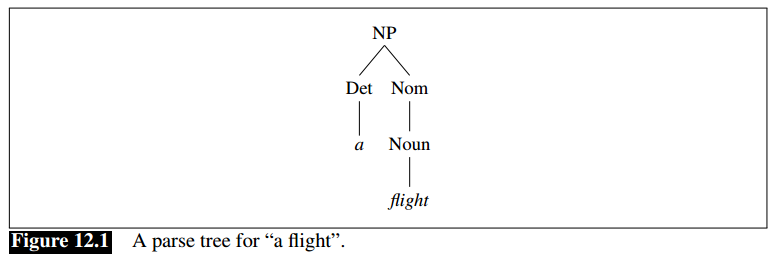
\includegraphics[scale = 0.5]{parse_tree.png}}
%\end{minipage}
%\caption{\footnotesize{\textbf{An example parse tree}. Each directed edge in the tree represent an derivation of an non-terminal symbol (node) to either an non-terminal symbol or a terminal symbol (node). A parent symbol dominates all descendant symbol. }}
%\label{fig: parse_tree}
%\end{figure}


\begin{figure}
\begin{minipage}[t]{1\linewidth}
  \centering
  \centerline{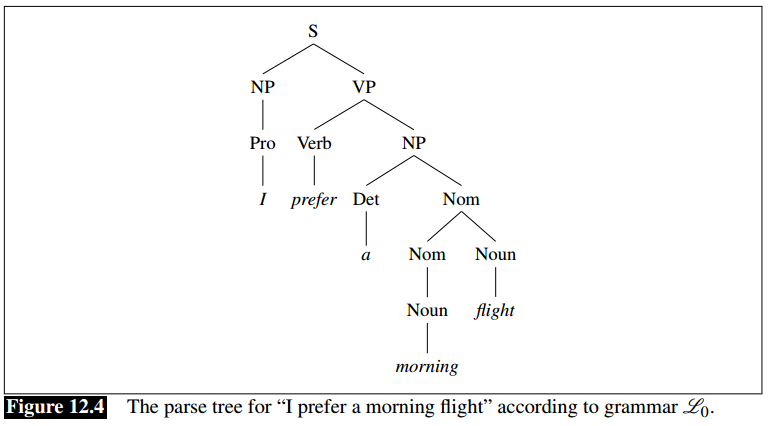
\includegraphics[scale = 0.5]{parse_tree_2.png}}
\end{minipage}
\caption{\footnotesize{\textbf{An example parse tree}.}}
\label{fig: parse_tree2}
\end{figure}

A CFG can be thought of in two ways: as a device for \emph{generating sentences} and as a device for \emph{assigning a structure} to a given sentence. As a generatior, we can view $"\rightarrow"$ as "{rewrite the symbol on the left with the string of symbols on the right}". This sequence of rule expansions is called a
\emph{\textbf{derivation}}  of the string of words. CFG can be represented in two ways:
\begin{itemize}
\item \emph{\textbf{parse tree}}. Because context-free rules can be hierarchically embedded,  we can combine the previous rules with others to build a tree-structure directed graph.  The \emph{formal} language defined by a CFG is the set of strings that are derivable from the designated \textbf{start symbol} (root). Each \emph{\textbf{grammar}} must have \emph{one} designated start symbol, which is often called \emph{S}. Since context-free grammars are often used to define sentences, S is usually interpreted as the “sentence” node, and the set of strings that are derivable from S is the set of sentences in some simplified version of English. Figure \ref{fig: parse_tree2} describes a grammar $\mathcal{L}_{0}$. We can use this grammar to \emph{generate sentences} of this “ATIS-language”. We start with S, expand it to NP VP, then choose a random expansion of NP (let’s say, to
I), and a random expansion of VP (let’s say, to Verb NP), and so on until we generate the string \emph{I prefer a morning flight}. 

\item  \emph{\textbf{bracketed notation}} here is the bracketed representation of the parse tree of Figure \ref{fig: parse_tree2}: $$[_{S} [_{NP} [_{Pro} \text{\textbf{I}}]] [_{VP} [_{V} \text{\textbf{prefer}}] [_{NP} [_{Det} \text{\textbf{a}}] [_{Nom} [_{N} \text{\textbf{morning}}] [_{Nom} [_{N} \text{\textbf{flight}}]]]]]]$$
\end{itemize}


A CFG like that of above defines a \emph{formal language}. A formal language is a set of strings. Sentences (strings of words) that can be derived by a
grammar are in the formal language defined by that grammar, and are called \emph{\textbf{grammatical}} sentences. Sentences that cannot be derived by a given formal grammar are not in the language defined by that grammar and are referred to as \textbf{ungrammatical}. In linguistics, the use of formal languages to model natural languages is called generative grammar since the language is defined by the set of possible sentences “generated” by the grammar. 

As seen above, CFGs are set of rules to define the constituent structure of natural languages, i.e. how the words are grouped and ordered to form a sentence. These rules can be used to define the domain of distribution of a given language.  CFG is a language model to generate formal languages. However, it does not care the meaning of the sentence. \emph{A language is defined through the concept of derivation}. One string derives another one if it can be rewritten as the second one by some series of rule applications.

\begin{itemize}
\item \textbf{syntactic parsing}: The problem of mapping from a string of words to its parse tree. 
\end{itemize}

\section{Grammar rules in English and some terminologies}
\subsection{English Sentence-Level Constructions}
There are several common sentence-level constructions:
\begin{itemize}
\item \textbf{declarative structure}:  Sentences with declarative structure have a subject noun phrase followed by a verb phrase. $"\text{S} \rightarrow \text{NP}\,\, \text{VP}"$. It is used to make \emph{statements} or \emph{assertions}. e.g.  "You are my friend."
\item \textbf{imperative structure}: Sentences with imperative structure often begin with a verb phrase and have no subject. $"\text{S} \rightarrow  \text{VP}."$ They are called imperative because they are almost always used for \emph{commands} and \emph{suggestions}.  e.g. "Be my friend!"
\item \textbf{interrogative structure}, i.e. yes-no question structure: Sentence typically raises a \emph{question}. Sentences with interrogative structure are often (though not always) used to
ask questions; they begin with an auxiliary verb, followed by a subject NP, followed by a VP.  $"\text{S} \rightarrow \text{Aux}\;  \text{NP}\,\,\text{VP}."$ e.g. "Are you my friend?"
\item \textbf{exclamative structure}, sometimes called an exclamatory sentence, typically expresses an exclamation;
\item \textbf{wh-question structure}: These are so named because one of their constituents is a \emph{wh-phrase}, that is, one that includes a \emph{wh-word} (who, whose, when, where, what, which, how, why). It includes \emph{wh-subject-question structure} and \emph{wh-non-subject-question structure}.
\begin{itemize}
\item \textbf{wh-subject-question structure} is identical to the \emph{declarative} structure, except that
the first noun phrase contains some wh-word. $"\text{S} \rightarrow \text{Wh-NP}\,\, \text{VP}"$. e.g. "What airlines fly from Burbank to Denver?"
\item \textbf{wh-non-subject-question structure}, the wh-phrase is not the subject of the sentence, and so the sentence includes another subject. In these types of sentences
the auxiliary appears before the subject NP, just as in the \emph{interrogative} structures. $"\text{S} \rightarrow \text{Wh-NP}\,\,\text{Aux}\,\,  \text{NP}\,\,\text{VP}."$ e.g. "What flights do you have from Burbank to Tacoma Washington?" This type of structure contains what are called \textbf{long-distance dependencies}  because the Wh-NP  is far away from the predicate that it is semantically related to, the main verb have in the VP. 
\end{itemize}
\end{itemize}

\subsection{The Noun Phrase}
An English noun phrase can have:
\begin{itemize}
\item \textbf{determiner}: Common kinds of determiners include \textbf{definite and indefinite articles} (like \textbf{the} and \textbf{a} or \textbf{an}), \textbf{demonstratives} (\textbf{this} and \textbf{that}), \textbf{possessive determiners} (\textbf{my} and \textbf{their})
\item \textbf{nominal}: The nominal construction follows the determiner and contains any pre- and posthead noun modifiers. 
\item \textbf{before the head noun}: A number of different kinds of word classes can appear \emph{before} the head  but \emph{after the determiner} (the \textbf{“postdeterminers”}) in a nominal. These include \textbf{cardinal numbers}, \textbf{ordinal numbers}, \textbf{quantifiers}, and \textbf{adjectives}. Adjectives can also be grouped into a phrase called an \emph{\textbf{adjective phrase}} or AP. APs can have an adverb before the adjective.
\item \textbf{after the head noun}:  A head noun can be followed by \emph{postmodifiers} such as \emph{prepositional phrases}, \emph{non-finite clauses}, \emph{relative clauses}. The three most common kinds of non-finite postmodifiers are the \textbf{gerundive (-ing), -ed, and infinitive forms}.
\begin{itemize}
\item \textbf{Gerundive postmodifiers}: i.e. -ing form;  e.g. "any flights [\emph{arriving after eleven a.m.}]" 
\item \textbf{non-finite clauses}: e.g. "She left the building [\emph{to find her friends}]"
\item \textbf{infinitives forms}: e.g. "I need to have dinner [\emph{served}]"
\item \textbf{-ed forms}: e.g. "Which is the aircraft [\emph{used by this flight}]?"
\item A \emph{postnominal \textbf{relative clause}} (more correctly a restrictive relative clause), is a clause that often begins with a relative pronoun (that and who are the most common). The relative pronoun functions as the subject of the embedded verb. e.g. "a flight [\emph{that serves breakfast}]"
\end{itemize}
\item \textbf{before the noun phrase}:  Word classes that modify and appear before NPs are called \textbf{predeterminers}. Many of these have to do with number or amount; a common predeterminer is "all".

\end{itemize}

\subsection{The Verb Phrase}
The verb phrase consists of the verb and a number of other constituents. 
\begin{align*}
\text{VP} &\rightarrow \text{Verb}\\
\text{VP} &\rightarrow \text{Verb}\,\,\text{NP}\\
\text{VP} &\rightarrow \text{Verb}\,\,\text{PP}\\
\text{VP} &\rightarrow \text{Verb}\,\,\text{NP}\,\,\text{PP} \\
\text{VP} &\rightarrow \text{Verb}\,\,\text{S}
\end{align*}
Many other kinds of constituents, such as an entire embedded sentence, can follow the verb. These are called \emph{\textbf{sentential complements}}, "$\text{VP} \rightarrow \text{Verb}\,\,\text{S}$".  Similarly, another potential constituent of the VP is another VP. This is often the case for verbs like "want", "would like", "try", "intend", "need": "Hi, I want $[_{\text{VP}}$ \emph{to arrange three flights}$]$"

While a verb phrase can have many possible kinds of constituents, not every verb is compatible with every verb phrase. This idea that verbs are compatible with different kinds of complements is a very old one; traditional grammar distinguishes between \emph{\textbf{transitive verbs}} like "find", which  take a direct object NP ("I found a flight"), and \textbf{\emph{intransitive verbs}} like "disappear", which do not ("I disappeared a flight"). We say that a verb like "find" \textbf{subcategorizes for} an NP, and a verb like "want" \emph{subcategorizes for} either an NP or a non-finite VP. We also call these constituents the \textbf{complements of the verb} (hence our use of the term \emph{sentential complement} above). So we say that "want" can take a \textbf{VP complement}. These possible sets of complements are called the \textbf{subcategorization frame} for the verb.

We can capture the association between verbs and their complements by making separate subtypes of the class Verb. Each VP rule could then be modified to require the appropriate \emph{verb subtype}. 
\begin{align*}
\text{VP} &\rightarrow \text{Verb-with-no-complement}\\
\text{VP} &\rightarrow \text{Verb-with-NP-comp}\;\,\,\text{NP}\\
\text{VP} &\rightarrow \text{Verb-with-S-comp}\;\,\,\text{S}
\end{align*}


\begin{figure}
\begin{minipage}[t]{1\linewidth}
  \centering
  \centerline{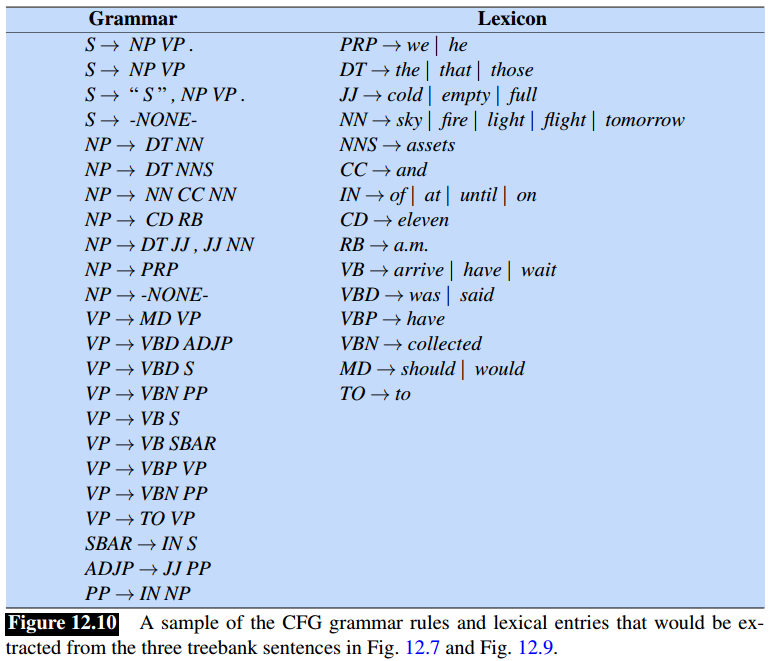
\includegraphics[scale = 0.5]{CFG_rules_treebank.png}}
\end{minipage}
\caption{\footnotesize{\textbf{An example CFG rules from treebank}.}}
\label{fig: parse_tree2}
\end{figure}

\subsection{Coordination}
The major phrase types discussed here can be conjoined with \textbf{conjunctions} like "and", "or", and "but" to form larger constructions of the same type. For example, a \textbf{coordinate} noun phrase can consist of two other noun phrases separated by a conjunction. e.g. "A and B". 

Note that the ability to \emph{form coordinate phrases through conjunctions} is often used as a \textbf{test for constituency}. The fact that these phrases can be conjoined is evidence for the presence of the underlying \emph{Nominal constituent} we have been making use of. $$\text{I need to know the }[_{Nom} [_{Nom}\text{ aircraft}]\text{ and} [_{Nom}\text{ flight number}]].$$

The rules for these constituents can be summarized as below:
\begin{align*}
\text{VP} &\rightarrow \text{VP}\,\,\text{and/or/but}\;\;\text{VP}\\
\text{S} &\rightarrow \text{S}\,\,\text{and/or/but}\;\;\text{S}\\
\text{NP} &\rightarrow \text{NP}\,\,\text{and/or/but}\;\;\text{NP}\\
\text{Normial} &\rightarrow \text{Normial}\,\,\text{and/or/but}\;\;\text{Normial}
\end{align*}



\section{Treebanks and Head-finding rules}
The syntactic constituents could be associated with a \textbf{lexical head}; N is the head of an NP, V is the head of a VP.  This idea of a head
for each constituent dates back to Bloomfield 1914, and is central to the \textbf{dependency grammars} and \textbf{dependency parsing}.

In one simple model of lexical heads, each context-free rule is associated with a \emph{head}. The head is the word in the phrase that is grammatically the most \emph{important}. \textbf{Heads are passed up the parse tree}; thus, each non-terminal in a parse tree is annotated with a single word, which is its \emph{lexical head}.
Figure \ref{fig: head_finding} shows an example of such a tree from Collins (1999), in which each non-terminal is annotated with its head.

\begin{figure}
\begin{minipage}[t]{1\linewidth}
  \centering
  \centerline{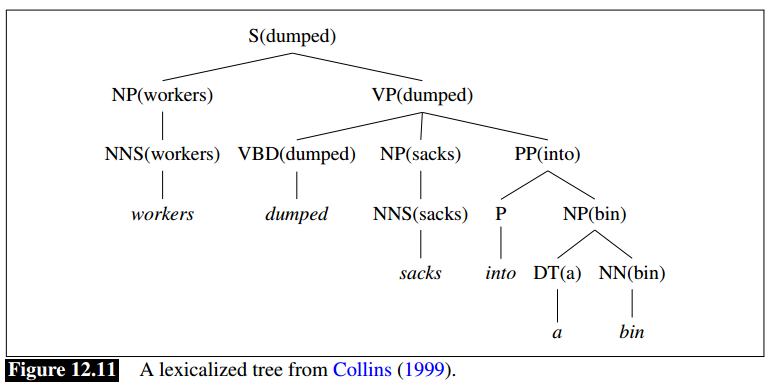
\includegraphics[scale = 0.5]{head_finding.png}}
\end{minipage}
\caption{\footnotesize{\textbf{An example head passing up to the tree}.}}
\label{fig: head_finding}
\end{figure}

For the generation of such a tree, each CFG rule must be augmented to identify \emph{one right-side constituent} to be the \textbf{head child}. The \emph{headword} for a node is then set to the headword of its head child. 

An alternative approach to finding a head is used in most practical computational systems. Instead of specifying head rules in the grammar itself, heads are identified
\emph{dynamically} in the context of trees for specific sentences. In other words, once a sentence is parsed, the resulting tree is walked to \textbf{decorate} each node with the appropriate head. 

Selected other rules from this set are shown in Figure \ref{fig: head_finding_rules}. For example, for VP
rules of the form $\text{VP} \rightarrow \text{Y}_1 \ldots \text{Y}_n$, the algorithm would start from the left of $\text{Y}_1 \ldots \text{Y}_n$ looking for the first $\text{Y}_i$ of type TO; if no TOs are found, it would search for the first $\text{Y}_i$ of type VBD; if no VBDs are found, it would search for a VBN, and so on.


\begin{figure}
\begin{minipage}[t]{1\linewidth}
  \centering
  \centerline{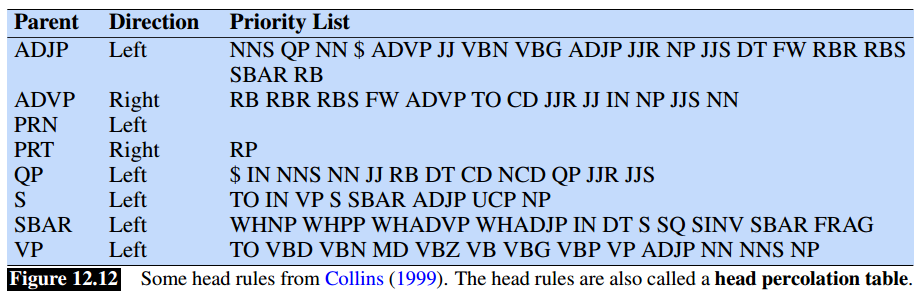
\includegraphics[scale = 0.5]{head_finding_rules.png}}
\end{minipage}
\caption{\footnotesize{\textbf{The rule for head-finding in a constituency tree}.}}
\label{fig: head_finding_rules}
\end{figure}

\section{Grammar Equivalence and Normal Form}
We can compare if two grammars are the same. We usually distinguish two kinds of grammar equivalence: 
\begin{itemize}
\item \textbf{strong equivalence}: Two grammars are strongly equivalent if they \emph{\textbf{generate} the same set of strings} and if they \emph{\textbf{assign} the same phrase structure} to each sentence (allowing merely for renaming of the non-terminal symbols). 
\item \textbf{weak equivalence}: Two grammars are weakly equivalent if they \emph{\textbf{generate} the same set of strings} but do \textbf{not} assign the same phrase structure to each sentence.
\end{itemize}
It is sometimes useful to have a \textbf{normal form} for grammars, in which each of the productions takes a particular form. 

\textbf{Chomsky normal form (CNF)}: for a context-free grammar to be CNF, if it is $\epsilon$-free and if in addition each production is either of the form $A \rightarrow B\;\; C$ or $A \rightarrow a$.  That is, the right-hand side of each rule either has \textbf{two non-terminal symbols} or \textbf{one terminal symbol}. CNF implies that the parsing tree is \textbf{binary tree} since it forms \textbf{binary branching}.

[\textbf{Theorem}]: \emph{Any context-free grammar can be converted into a weakly equivalent Chomsky normal form grammar}.

The generation of a symbol A with a potentially infinite sequence of symbols B with a rule of the form $A \rightarrow A\;\; B$ is known as \textbf{Chomsky-adjunction}.
\newpage
\bibliographystyle{plainnat}
\bibliography{book_reference.bib}
\end{document}